\chapter{Project Plan}

\label{Chapter5} For referencing this chapter elsewhere, use \ref{Chapter5}

\lhead{Chapter 5. \emph{Project Plan}}

%----------------------------------------------------------------------------------------
%	SECTION 1
%----------------------------------------------------------------------------------------

\section{Project Schedule}

The schedule of the project will consist of a list of tasks along with their estimated time. The best representation in order to output a graphical representation of those tasks and their deadline is to use a \emph{Gantt Chart}. This chart enables a graphical representation of the plan along with the allocated resources for each one of the tasks. This will allow to identify the critical path of the project - the sequence of tasks from beginning to end that takes the longest time to complete, any delay on one of the tasks of the sequence will automatically delay the whole project.

The tasks that will need to be completed by the end of the dissertation are the following:

\begin{itemize}
  \item Appropriation of the FPGA hardware architecture
  \begin{itemize}
    \item Basic actions
    \item Complete cycle
    \item Higher-level implementation
  \end{itemize}
  \item Appropriation of the CNN
  \begin{itemize}
    \item Basic implementation
    \item Parameter tuning
    \item Optimisation implementation
  \end{itemize}
  \item Combination of the CNN and FPGA
  \item Backend software
  \begin{itemize}
    \item Coordination between the two elements (hardware and network)
    \item Security rules
  \end{itemize}
  \item Experimentation guidelines
  \item Experimentation results
  \item Results Evaluation
  \item Dissertation writing
  \begin{itemize}
    \item Abstract
    \item Chapter 1 - Introduction
    \item Chapter 5 - Implementation
    \item Chapter 6 - Results
    \item Chapter 7 - Discussion
    \item Chapter 8 - Evaluation and Future Work
    \item Chapter 9 - Conclusion
  \end{itemize}
\end{itemize}

A Gantt chart has been created in order to comply with the fact that the final draft will have to be done by Friday 17/07. Backtracking from there, the other tasks and their associated resources can be viewed as follows.

\begin{figure}[htbp]
	\centering
		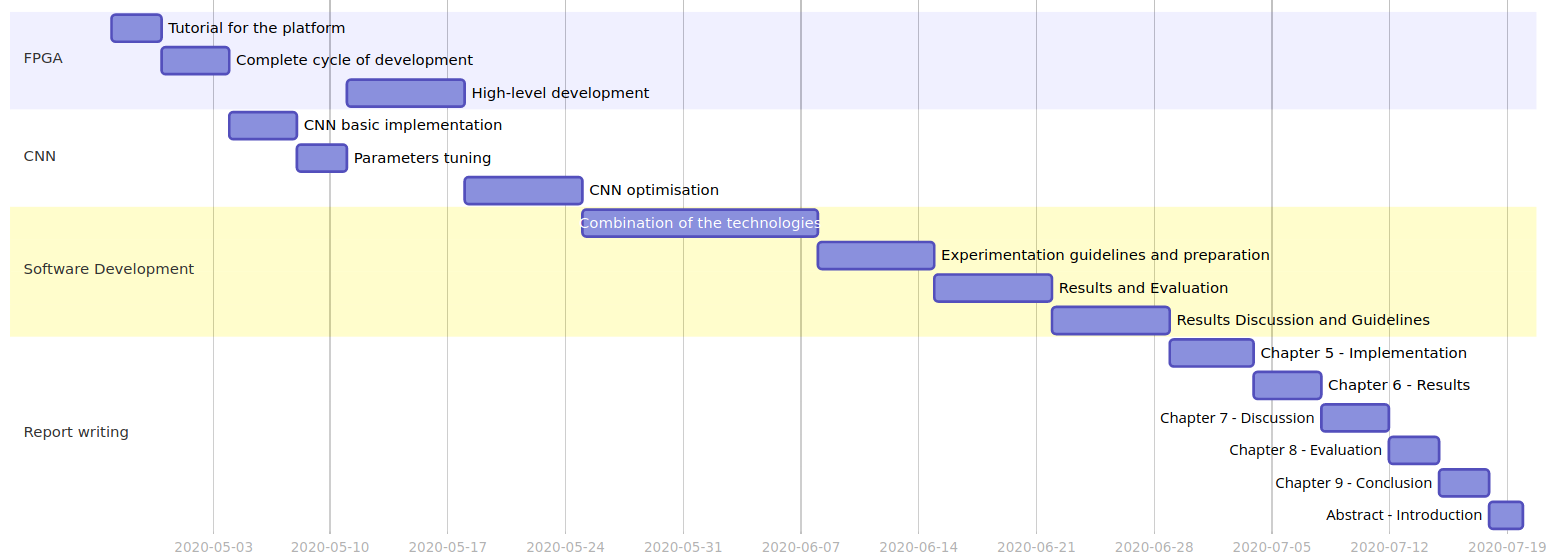
\includegraphics[width=16cm]{Figures/gantt.png}
	\caption[Gantt Chart]{Gantt chart for the project}
	\label{fig:gantt}
\end{figure}

%----------------------------------------------------------------------------------------
%	SECTION 2
%----------------------------------------------------------------------------------------

\section{Supporting Plans and Risk Management}


The following project will be developed during an internship and will enable a loop of direct feedback from what I produce to the supervisors. The internship will help me produce a quality project as I will have to work by the side of my supervisors. If the subject will need me to learn new technologies and to implement a state-of-the-art application with them, I believe the environment will help me do so.

What risks are there?

How likely are there to occur?

What will their impact be?

How can we minimise their occurrence?
